\documentclass[a4paper,10pt]{article}
% abstract + title + authors
\usepackage{abstract}
\renewcommand{\abstractnamefont}{\normalfont\bfseries}
\renewcommand{\abstracttextfont}{\normalfont\small\itshape} 
\usepackage{titlesec}
\usepackage{authblk}
\usepackage{datetime}
\usepackage{afterpage}
\usepackage{caption}
\usepackage{subcaption}
\usepackage{hanging}
\usepackage{setspace}

\newdateformat{usvardate}{
\monthname[\THEMONTH] \ordinal{DAY}, \THEYEAR}

% keywords
\providecommand{\keywords}[1]{\textbf{\textit{Keywords---}} #1}

% math
\usepackage{amssymb}
\usepackage{newtxmath}

% manuscript looking document
\usepackage{setspace}
\usepackage{lineno,xcolor}
\setlength{\parskip}{0.5em}

% comments
\usepackage[draft]{todonotes}

% graphics
\usepackage{graphicx}
\usepackage{float}

% references & links
\usepackage[
backend=biber,
style= authoryear,
citestyle = authoryear,
url=false,
doi=true,
isbn=false
]{biblatex}
\addbibresource{../references.bib}

\usepackage{hyperref}
\hypersetup{
    colorlinks=true,
    citecolor=magenta,
    linkcolor=magenta
}
\usepackage{doi}
\graphicspath{ {./figures/} }

\begin{document}

% title
% Article title
  \title{{\normalsize Attachment 1} \\
	{\LARGE \textsc{Structural controlability of pollination networks}}}

% Authors and Affiliations
  \author{\large E. Fernando Cagua}
  \author{\large Kate Wootton}
  \author{\large Anna J. Voinopol Sassu}
  \author{\large Daniel B. Stouffer}
  \affil{\normalsize Center of Integrative Ecology, School of Biological Sciences, University of Canterbury}
 
\date{}
\maketitle

% line numbers
\linenumbers
\setlength\linenumbersep{15pt}
\renewcommand\linenumberfont{\normalfont\footnotesize\sffamily\color{gray}}

\doublespacing
 
\section*{Introduction}

Ecological communities are formed by the interconnection of several species. Therefore, changes in the abundances of one species can potentially alter the abundances of the species they interact with. For instance, in a classic example of ecosystem cascades, a reduction on the abundance of sea otters, an important predator or sea urchins, can drive a dramatic reduction on kelp abundances because the sea urchins that consume kelp are released from predation. It has been long established that some species, like the sea otter, have a disproportionate large effect in their environment relative to their abundance. 

In several ecosystems the relative importance of species have been identified based on empirical observations of long term dynamics. However, in less studied, highly diverse, or where the "keystone" role is shared by several species, it can be challenging to determine which is the set of species that influence the most the ecosystem dynamics. Alternative approaches that recognize a continuum of importance and that are less dependent on empirical observations have also been developed. Some of them are based on metrics that evaluate their position in the food web or on mass balance models of functional groups. Nevertheless, these approaches are conceptually limited to throphic interactions and in general ignore the structural mechanisms that allow or prevent the spread of perturbations in the ecosystem.

From a systems perspective, perturbations like over-exploitation, eutrophication or global warming are equivalent to management actions like culling, no-take areas or captive rearing in the sense that they have the potential to modify the abundances of one or several species in the ecosystem. Therefore identifying these key species is crucial not only to predict how these perturbations will spread trough the community but also to guide effective conservation efforts.

Recent work on the control of complex systems suggest that in principle it is possible to alter any ecological community's composition, by modifying the abundances of just some key species \autocite{Isbell2013, Cornelius2013}. Here, we apply these theories to estimate the controllability of different ecological communities and to find driver species: species, that due to the structural characteristics of their interactions are more likely to drive the dynamics of the community.

Invasive species have been shown to have a disproportionate effect on the structure of pollination communities. Influencing for example the strength of species interactions, and the degree of network nestedness and connectivity \autocite{Olesen2002, Aizen2008, Bartomeus2008, Vila2009, Traveset2013}. However whether this influence is translated into a driver role has not been tested. Here we use plant pollinator communities to investigate the number of species that should be managed to control population dynamics of the whole community, the characteristics that determine whether a species should be managed or not and how invasive species fit. 

\section*{Methods} 

To investigate the dynamic controllability of pollination networks, we used ten paired plants-pollinator communities. Each par was composed by a community invaded by a plant and a community free of the invasive species. Weighted visitation networks were constructed from previously published visitation data collected from pollination communities in Bristol, Great Britain \autocite{Lopezaraiza-Mikel2007} and the National Cap de Creus in Northeastern Spain \autocite{Bartomeus2008}. The four British uninvaded communities the non-invaded plots were obtained by experimentally removing the invasive species \textit{Impatients grandulifera} (\hyperref[fig:photographs]{Figure \ref{fig:photographs}a}). Contrastingly, Spanish uninvaded communities were obtained from plots that were not been colonised by the invasive species \textit{Carpobrotus affine acinaciformis} or \textit{Opuntia stricta} (\hyperref[fig:photographs]{Figure \ref{fig:photographs}b, c}). In each of the networks we calculated the minimum number of driver species---species that need to be managed in order to gain full control of the community.

\begin{figure}
    \centering
    \begin{subfigure}{0.3\textwidth}
        \centering
        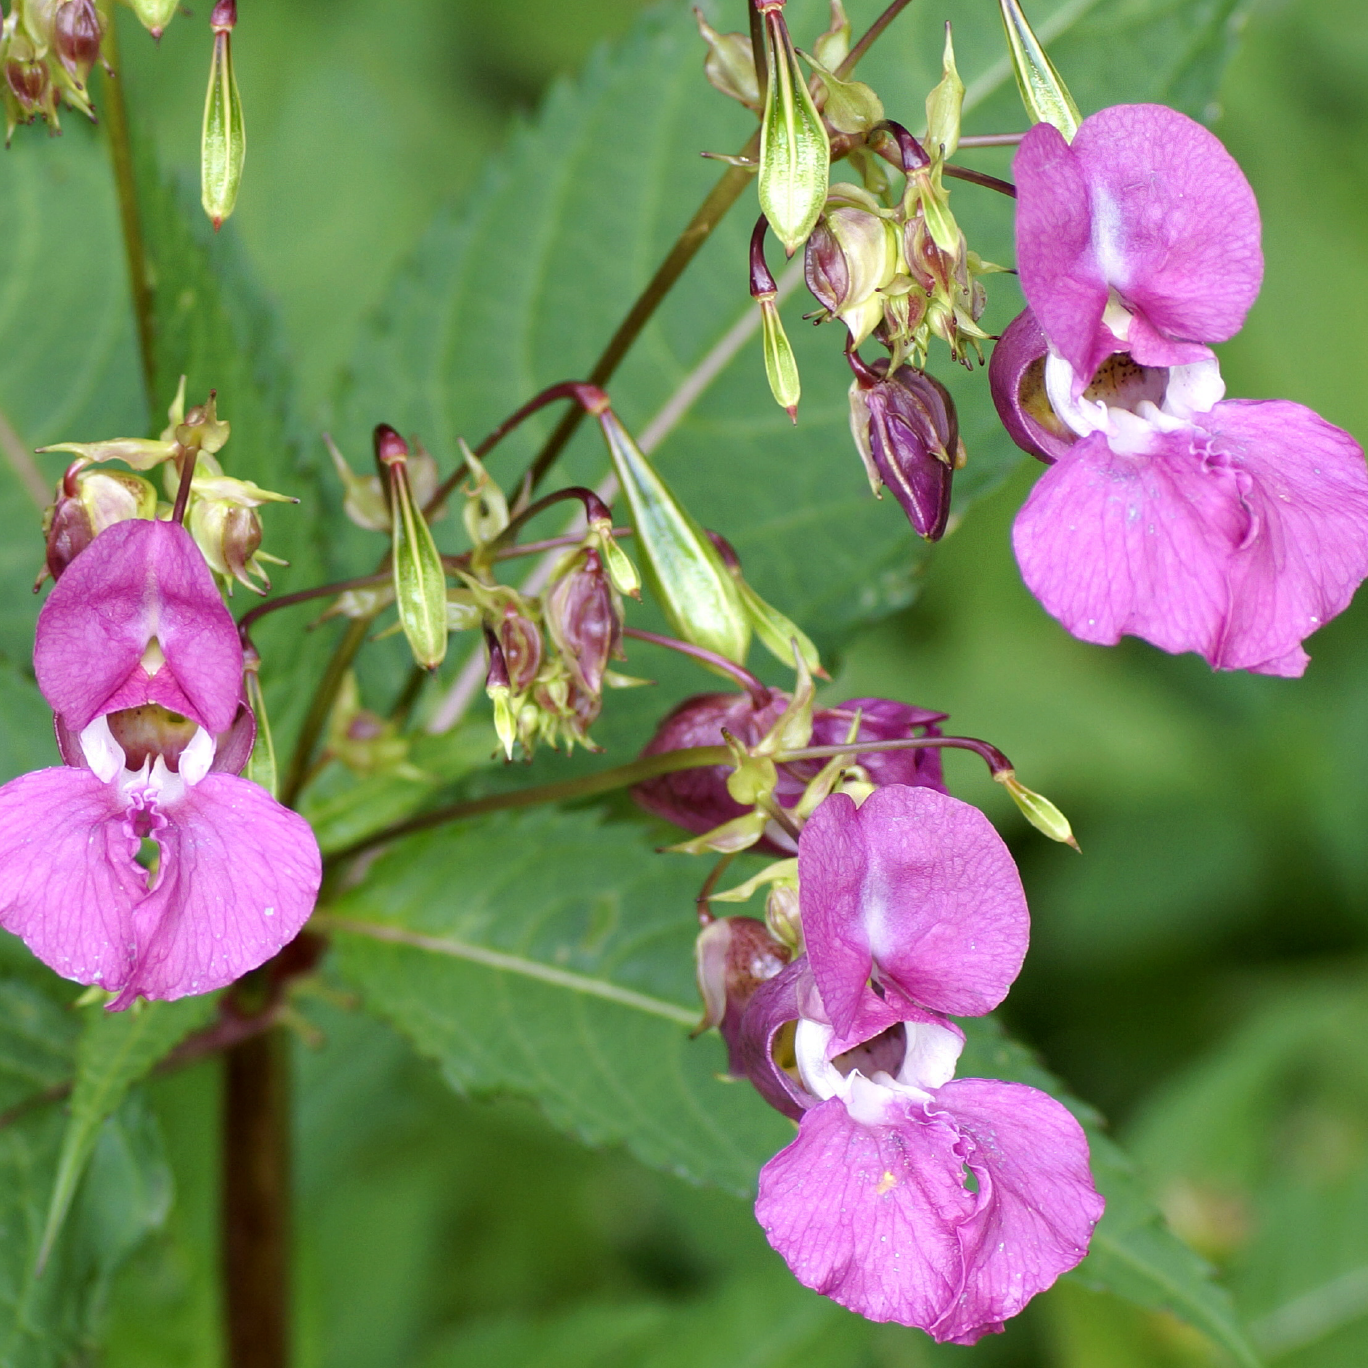
\includegraphics[width=\textwidth]{Impatiens_glandulifera}
        \caption{\textit{Impatiens glandulifera}}
    \end{subfigure}
    \hfill
    \begin{subfigure}{0.3\textwidth}
        \centering
        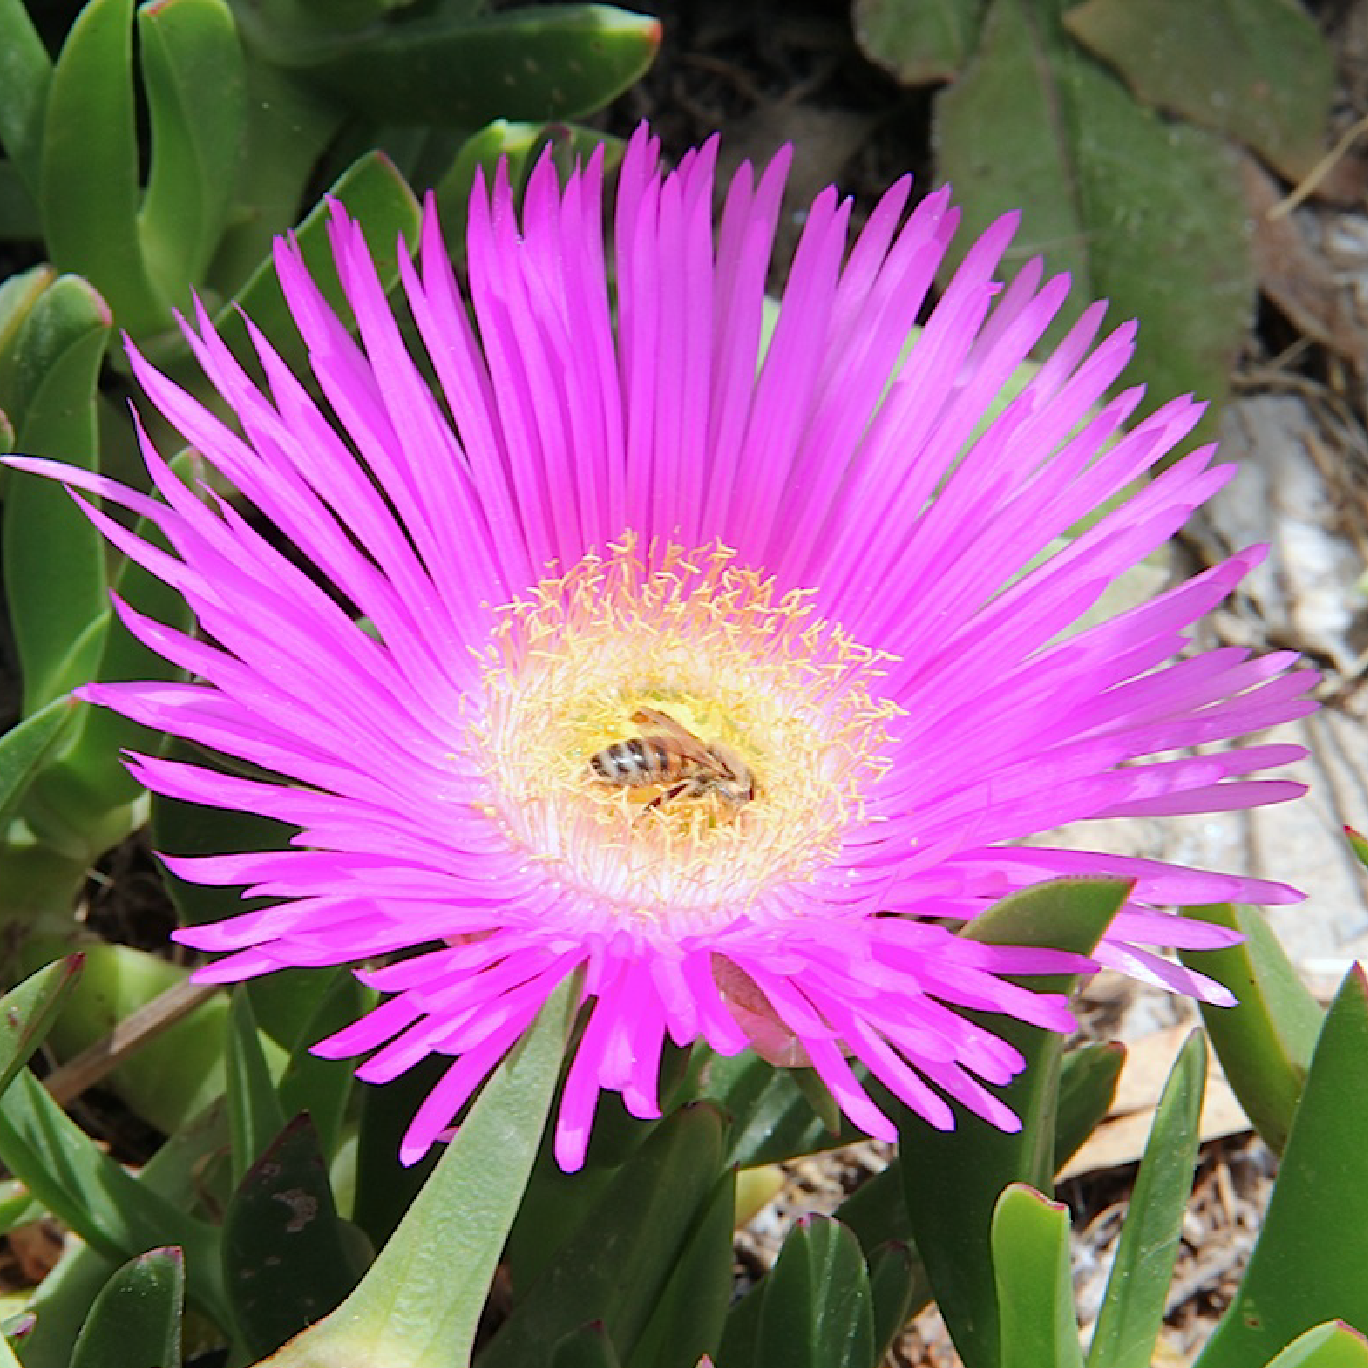
\includegraphics[width=\textwidth]{Carpobrotus_acinaciformis}
        \caption{\textit{Carpobrotus acinaciformis}}
    \end{subfigure}
    \hfill
    \begin{subfigure}{0.3\textwidth}
        \centering
        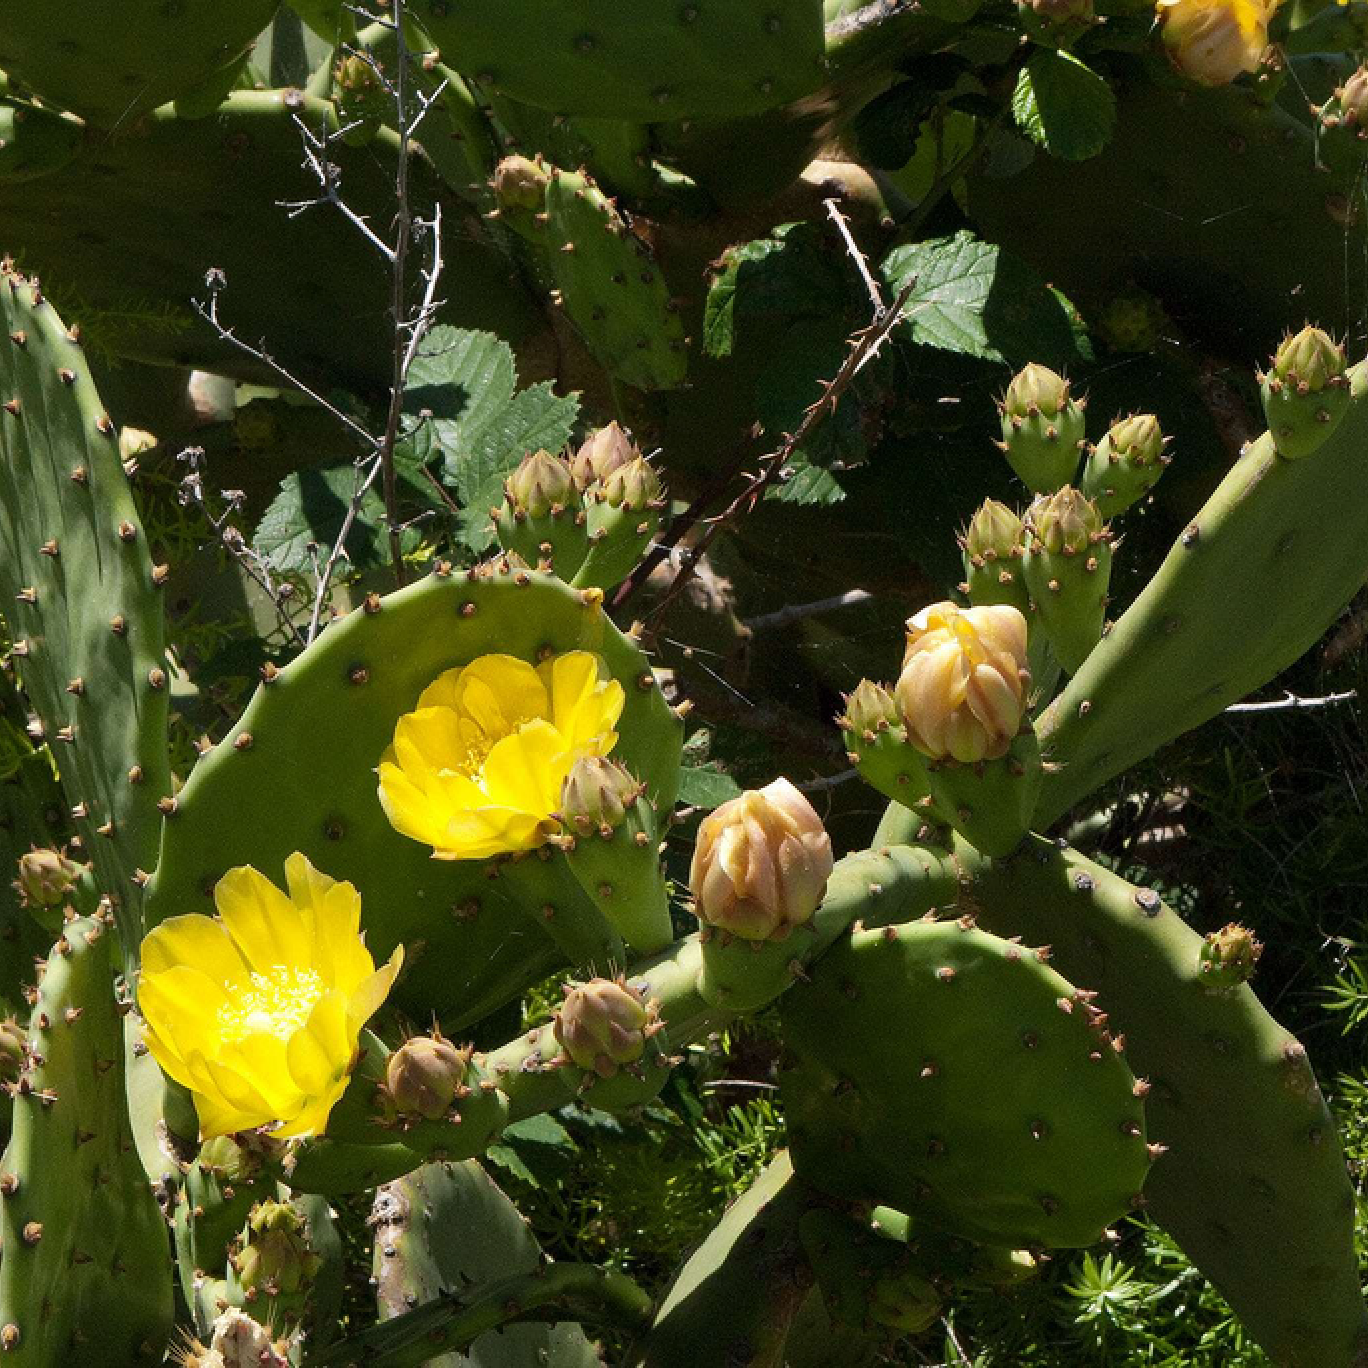
\includegraphics[width=\textwidth]{Opuntia_stricta}
        \caption{\textit{Opuntia stricta}}
    \end{subfigure}
    \hfill
    \caption{
    Invasive species present in the studied pollination communities (photographs by \href{https://commons.wikimedia.org/wiki/File:Impatiens_glandulifera_Royle_(7677070626).jpg}{Udo Schmidt}, \href{https://commons.wikimedia.org/wiki/File:Carpobrotus_acinaciformis_pm.jpg}{Peter Mansfeld}, and \href{https://www.flickr.com/photos/tony_rodd/5265326818}{Tony Rodd}).
    }
    \label{fig:photographs}
\end{figure} 

We first assigned a direction to each link between plants and pollinators given by the direction of dependency. For each link between a plant and its pollinator we quantified the level of dependency of the plant on the pollinator and vice versa \autocite{Bascompte2006}. The link points to the plant if the its dependency on the pollinator is larger than the pollinator's dependency on the plant. The dependency of plant $i$ on pollinator $j$ is the ratio between the visits coming from pollinator $j$ and all pollinator visits to plant $i$. The dependency of pollinator $j$ on plant $i$ is the ratio of the visits by pollinator $j$ to plant $i$ and all visits of pollinator $j$. 

In a directed network, a matching is a subset of links in which no two links share a common starting species or a common ending species. A species is matched if it is an ending node of an link in the matching. Otherwise, it is unmatched. It has been shown that the number of driver species can be calculated by counting the number of unmatched nodes in the directed graph representation of the pollination network \autocite{Liu2011}. We then found a maximum in the an alternative bipartite representation of the pollination network \autocite{Csardi2006} (\autoref{fig:maximum_matching}). 

\begin{figure}
    \centering
    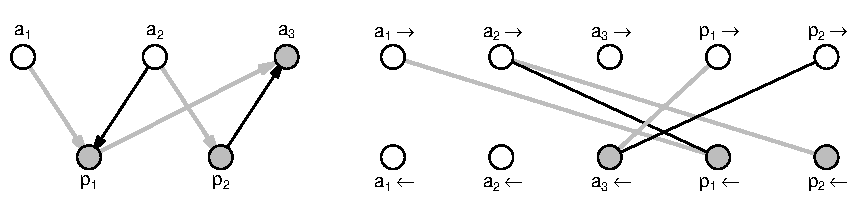
\includegraphics[width=\textwidth]{control_net}
    \caption{
    On the left a simple pollination network; the direction of the arrows indicates the direction of the largest dependency between species pairs. On the right the representation of the network used to calculate the maximum matching (in grey). Matched species, i.e. those whose dynamic could be ``controlled'' by another species are shown in blue. Note that the maximum matching is not necessarily unique.
    }
    \label{fig:maximum_matching}
\end{figure} 

We calculated dependencies based on visitation frequency, which has been shown to be an appropriate surrogate of the inter-specific effects \autocite{Bascompte2006, Vazquez2005}. However, because the degree distribution, and ultimately the number of driver species, can be affected by the sampling method \autocite{Bluthgen2010} we compared the number of driver species in a pollination community in which both visitation frequency and effectiveness were measured \autocite{Ballantyne2015}.

To quantify to what extent the number of driver species is characteristic of the structure of pollination networks we compared them a suit of random null-models. A set of null models were based on network randomisations that maintained the degree of plants, pollinators, and both plants and pollinators. To analyse the effects of the chosen directionality, we devised a null model in which we randomised the visitation patterns and re-calculated the new dependencies. In all cases we computed 999 randomisations.

We quantified the relative importance of each species for network dynamics. To do this, we counted the number of times a particular species was a driver species across all possible maximum matchings in the pollination network. The number of maximum matchings were found by generating the line graph of the alternative bipartite network representation (\autoref{fig:maximum_matching}), and then enumerating the maximal cliques in the complement of the line graph \autocite{Csardi2006}. 

Finally, we tackled the question whether some structural properties can predict the relative importance of driver species. Here, we regressed the importance of each species against measures of centrality (degree, betweenness), measures related to network robustness (contribution to nestedness) and measures of strength of association (visitation levels). 

\section*{Preliminary results} 

To date only data from the National Cap de Creus in Northeastern Spain has been analysed. We found that if we were to control the dynamics of the whole community, we would need to control between 55 and 75\% of the species in the community. The proportion of driver species did was not significantly different between invaded and uninvaded ecosystems. 

\iffalse
\begin{figure}
    \centering
		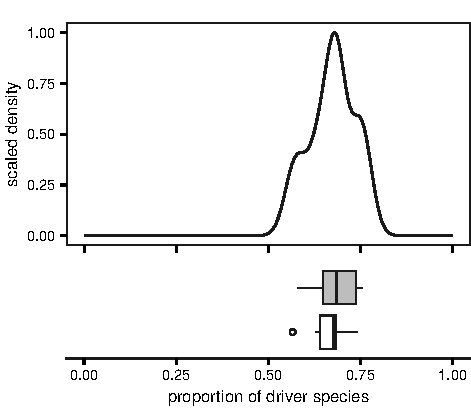
\includegraphics{n_driver}
    \caption{
    Proportion of species that needs to be controlled for all networks. There are no significant differences between invaded (grey box plot) and uninvaded (white box plot) communities.
    }
    \label{fig:n_driver}
\end{figure} 
\fi

Empirical pollination networks to randomisations have need significantly more driver species than randomisations that maintain the number of interacting species per plants. However when the number of interacting species is maintained in pollinators or in all species, the difference disappear (\autoref{fig:random_degree}). This suggest that the number of driver species is determined by the degree distribution of the species, in particular pollinators. This is consistent to previous findings that highlight the influence of the degree distribution on the controlability of complex networks \autocite{Liu2011, Benavides2015}. 

\begin{figure}
    \centering
		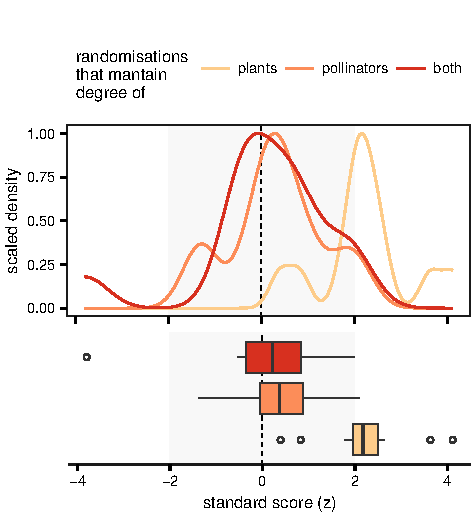
\includegraphics{random_degree}
    \caption{
    Difference between the number of driver species in the empirical pollination networks versus randomisations of the same networks. The unshaded area ($z < -2 , z > 2$) suggest a significant difference at a significance level of $\alpha = 0.05$.
    }
    \label{fig:random_degree}
\end{figure} 

However, when we compared the empirical networks to randomisations that maintain the network structure but shuffle the directionality of the dependency, we found that empirical networks need substantially more driver species than the random counterpart (\autoref{fig:random_direction}). This highlights the importance of asymmetries in structuring pollination networks. 

\begin{figure}
    \centering
		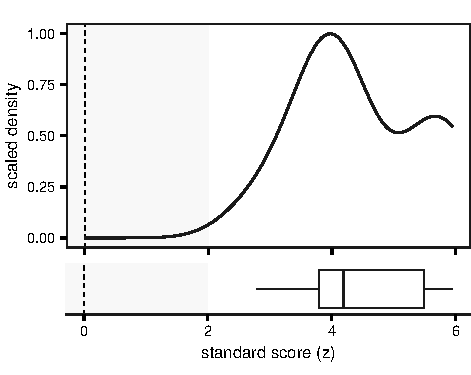
\includegraphics{random_direction}
    \caption{
    Difference between number of driver species in the empirical networks versus randomisations of the dependencies in the same networks. The unshaded area ($z > 2$) suggest a significant difference at a significance level of $\alpha = 0.05$.
    }
    \label{fig:random_direction}
\end{figure} 

Not all species have the same importance for network control. Pollinators in general seem to have a moderate-high role on driving the dynamics of other species. Plants on the other hand seem to be a skewed distribution, with some species having a very low and some species having a very high relative importance (\autoref{fig:per_guild}). 

\begin{figure}
    \centering
		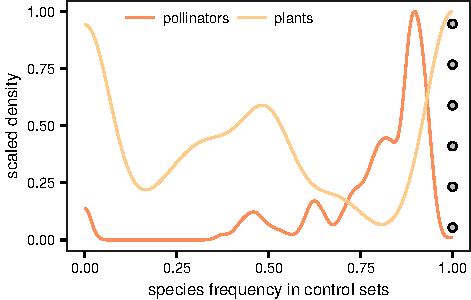
\includegraphics{per_guild}
    \caption{
    Distribution of the relative frequency a species is present in the set of driver species. Invasive species are depicted as grey points.
    }
    \label{fig:per_guild}
\end{figure} 

When looking at the relative importance of invasive species we found that, in all of the six analysed networks, they all have the maximum importance. They are certainly not unique in this regard, but it is remarkable that invasive species integrate this way in the community.

\section*{Acknowledgmenets}

The authors thank Dr. Takeuki Uno for the insight provided to find the set of all maximum matching algorithms, and Bernat Bramon and Marilia Gaiarsa for feedback in early stages of the project. EFC acknowledges the support from the University of Canterbury Doctoral Scholarship, the University of Canterbury Meadow Mushroooms Postgraduate Scholarship, a travel grant from the European Space Agency and a Rutherford Discovery Fellowship (to DBS). DBS ackloledges the support of a Rutherford Discovery Scholarship, administered by the Royal Society of New Zealand.

\printbibliography



\end{document}